%% This is emulateapj reformatting of the AASTEX sample document
%%
\documentclass[iop]{emulateapj}
\begin{document}

\title{Fate Of Stars at sun's location in the disk of Andromeda}

\author{Rafia Bushra}
\affil{Astronomy Department, University of Arizona}

\begin{abstract}
    % 1. A sentence that defines the topic
    % 2. A sentence that says why the topic is important
    % 3. A sentence that says what question you are exporing 
    % 4. A sentence about why that question is important
    % 5. A sentence that states what you found
    % 6. A conclusion about what your finding means.
    % The rest of the report should expand on each of the above bullet points in the abstract. Follow the below guidelines.
    
    In this paper, we present our findings from our simulation of life of sun-like stars in Andromeda galaxy's disk. By studying the fate of sun-like stars, we can get an understanding of stars in our own galaxy and of what happens to sun-like stars over time and during mergers. Using the simulation data, we studied the position and kinematics of Sun Analogs as a function of time and focused on a few interesting times in particular. This is important because studying position and kinematics can reveal the fate of sun-like stars by answering questions such as whether these stars remain bound to the galaxy, whether they end up in a different galaxy in the local group, what their trajectory is over time etc.      
\end{abstract}

\section{Introduction}

    % Define the topic you are studying and state why it matters. Overview our current understanding of the topic.
    % What are the open questions? Cite at least 3 journal papers.
    The Milky Way and Andromeda are the largest galaxies in the local group that is comprised of about 40 other much smaller galaxies. These two galaxies are quite similar in various aspects. They are similar in size, are both spiral, barred galaxies and have comparable mass $(M_{M31}\approx 1.6M_\odot)$. These two galaxies are also approaching each other with a velocity of $120kms^-1$ (Cox \& Loeb 2008 \cite{cl08}). M31 being one of the nearest galaxies and given all these similar properties, it is a very important object to study. Thus, studying the evolution of the Andromeda (M31) - Milky Way (MW) system, their pre-merger and post-merger conditions, fate of their stars etc. are of great significance. \medskip
    
    Our star system, the solar system lies about 8 kpc away from the center of our galaxy, Milky Way. At this distance from the galactic center, sun formed about 4.5 billion years ago and did not become unbound. It orbits the galactic center with an average speed of about 220 km/s. An interesting topic of stud is the fate of our sun as the galaxy evolves and eventually merges with Andromeda. Currently, there are few studies going on regarding this topic. Some inspiring ones are by Cox \& Loeb \cite{cl08} and Marel \& Besla \cite{marel}, where they simulate the evolution of sun like star in Milky Way's disk. Using their study as guideline, for this paper, we studied the fate of sun-like stars in Andromeda's disk. We also compare our findings to their \cite{cl08} \cite{marel} results to obtain a better understanding of sun-like stars. \medskip
    
    
\section{This Project}

    % State what question(s) you are exploring
    % Why is each question interesting/important? Relate back to intro.
    
    As we discussed in the previous section, for this project, we explore the evolution of sun-like stars in the disk of Andromeda. We are going to investigate the future trajectory of these stars by studying their position and kinematics over the next 12 billion years. Studying the position and kinematics of sun-like stars in M31 is interesting because it give us an outlook into our own evolution. We are also going to explore their conditions at some particular times of interest, especially before and after the merger takes place. These times of interest were chosen from the following plot: \medskip
    
    \begin{figure}[h]
        \centering
        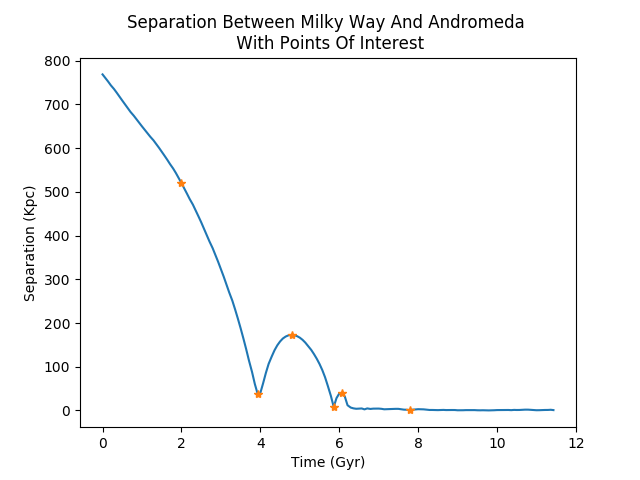
\includegraphics[width=\columnwidth]{separation}
        \caption{Separation between M31 and MW as function of time. The '*' symbols on the plot indicates the times we are interested in and will be working with.}
        \label{fig:separation}
    \end{figure}
    
    This is a plot of the separation between MW and M31 over the next 12 billion years, created using a simulation by Marel & Besla \cite{marel} which is described in the next section. From this plot, it can be noted that there are two close encounters and a third encounter after which the two galaxies merge. The times that we are interested in are marked by a '*' on the plot. We found these times interesting because of the events they are associated with, specially before and after events, so that we can compare. The times we chose are: 2 billion years from now which happens before any close encounters and is seperated by 520 kpc, 3.93 billion years from now when the first close encounter takes place and has a separation of 38 kpc, 4.79 billion years from now which is post-first-encounter and has a separation of 172 kpc, 5.86 billion years from now which is the second close encounter with a separation of 8 kpc, 6.07 billion years from now which is post-second-close-encounter and has a separation of 39 kpc, and finally, 7.79 billion years from now, which is after the merger when the separation is ~0 kpc, i.e. no separation. We didn't choose the the third close encounter because it is the merger and from that point on, the remains a constant (no separation). So we thought it would be better to choose a point that happens some time after the merger, when it has become more stable. We compare the conditions during these evens to present conditions, when the separation is 769 kpc. \medskip
    
    Some other questions that we will be exploring in this project is if any of the stars that started out at sun's location becomes unbound or not. If they do, what fraction of the candidates we chose becomes unbound? We will also be exploring if these stars end up in a different galaxy (MW). This is interesting because it informs us of the likelihood of the sun or a star like it to be bound to its galaxy or if they end up in a different galaxy. 

\section{Methods}

    % Write a paragraph that describes the simulation you are using. Details can be found in: van der Marel, Besla +2012 ApJ 753
    % Describe the code you wrote. What equations did you use? At least one component of the code must be unique to you (you can’t only use code from homework and in class labs - but you can use the solutions as a starting point to create your code).
    
    Our research heavily depends on the semi-analytic simulation of future motions of the MW, M31 and M33 due to their mutual gravitational interaction \cite{marel}. For this simulation, they approximated each galaxy as a constant one-component gravitational potential given by a Hernquist mass profile. They used equations of motion for the Center of Mass (COM) of each galaxy and integrated over all particles to properly calculate the gravitational attraction. They also accounted for dynamic friction by using the Chandrasekhar formula. All calculations were done assuming all the galaxy's mass is concentrated at the COM. For more details regarding the simulation we used, please refer to section 2.2 of the Marel & Besla paper \cite{marel}. \medskip
    
    The simulation produced the future positions (x, y and z coordinates) and velocities (vx, vy and vz components) of all the halo, disk and bulge particles in MW, M31 and M33 galaxies. There are two versions of this simulation: a high resolution version and a low resolution one. For this project, we chose disk particles of M31 from the high resolution simulation. We chose high resolution because it accounts for more particles and for this project, we need a high number of samples for better statistical analysis. These six parameters (x, y, z, vx, vy, vz) of all particles are calculated for the next 12 billion years, presented in 800 "snapshots". Each snapshot corresponds to a particular point in time. \medskip
    
    \begin{figure}[h]
        \centering
        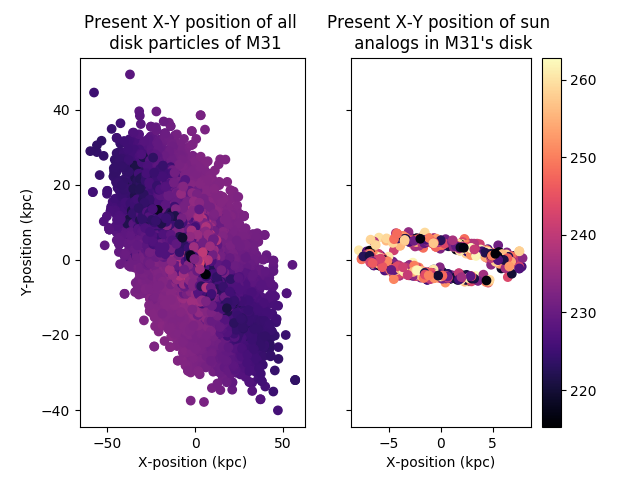
\includegraphics[width=\columnwidth]{masking}
        \caption{Particles chosen according to position and velocity constraints. Colorbar represents equatorial velocity of particles}
        \label{fig:separation}
    \end{figure}
    
\section{Results}
    
    % 1. Include at least two plots (with proper labels and figure captions). 
    % 2. Describe what your code returned. What did you find? Describe what is in the plot.
    
    \begin{figure}[h]
        \centering
        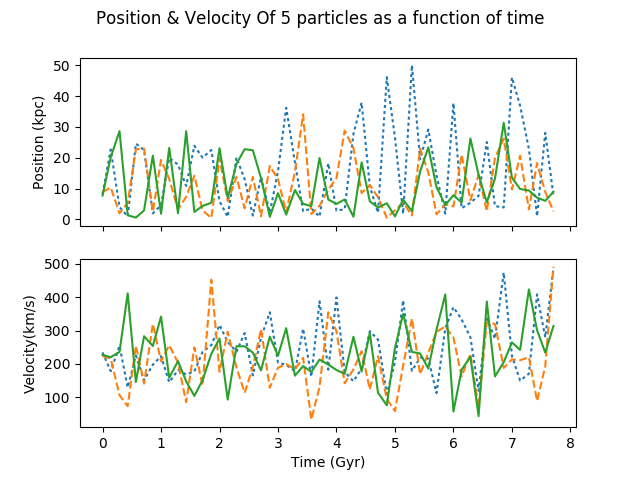
\includegraphics[width=\columnwidth]{trajectory}
        \caption{Motion and kinematics of 3 sun-like particles chosen randomly.}
        \label{fig:separation}
    \end{figure}
    
    \begin{figure}[h]
        \centering
        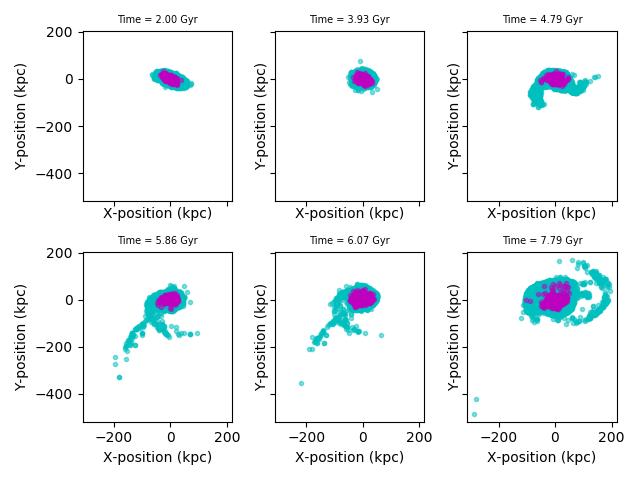
\includegraphics[width=\columnwidth]{snapshots}
        \caption{Position mapping of all particles at desired times}
        \label{fig:separation}
    \end{figure}
    
    \begin{figure}[h]
        \centering
        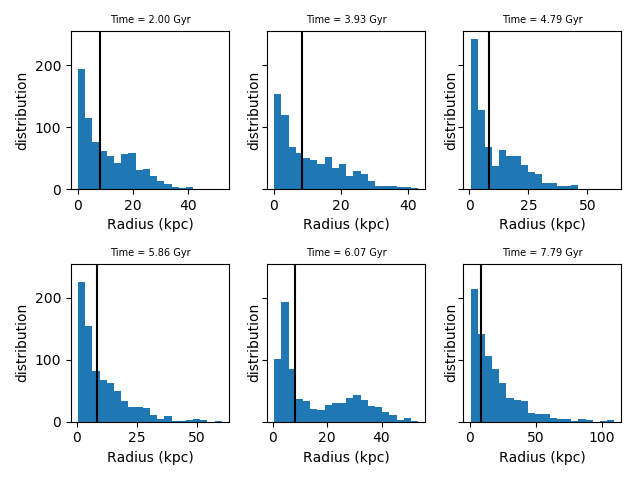
\includegraphics[width=\columnwidth]{histograms}
        \caption{Particle distribution at desired times}
        \label{fig:separation}
    \end{figure}
    
    

\section{Discussion}

    What did you learn? What do your results mean? What is the importance of your results ?

\section{Conclusion}

    1. Summarize your report - i.e expand a bit on each line of the abstract.
    2. Comment on future directions - what other things could you do to explore the topic further?

\begin{thebibliography}{}

    \bibitem{cl08}
        Cox, T. J., and Abraham Loeb. “The Collision between the Milky Way and Andromeda.” 
        \textit{Monthly Notices of the Royal Astronomical Society}, 
        vol. 386, no. 1, 2008, pp. 461–474., doi:10.1111/j.1365-2966.2008.13048.x.
    
    \bibitem{marel}
        Marel, Roeland P. Van Der, et al. “The M31 Velocity Vector. Iii. Future Milky Way M31-M33 Orbital Evolution, Merging, And Fate Of The Sun.” 
        \textit{The Astrophysical Journal}, 
        vol. 753, no. 1, 2012, p. 9., doi:10.1088/0004-637x/753/1/9.
    
\end{thebibliography}

\clearpage

\end{document}

